\subsection{Content Management Overview}

\subsubsection{Introduction}

When people hear the word `Content Management' a common reaction is:
``Oh no not another buzz word!"  Then they mentally switch off, freak
out or have some other reaction that doesn't end in understanding.
The purpose of this document is to change that.  Understanding what
content management is, is very easy.  It is the combination of two
concepts you probably already know about.  Content Management at it's
essence is the combination of a file system with a database table.  A
file system is just the place where you have been saving your
documents for years, all those files and folders on your C: drive!
  
\begin{figure}[h!]
  \centering
  \fbox{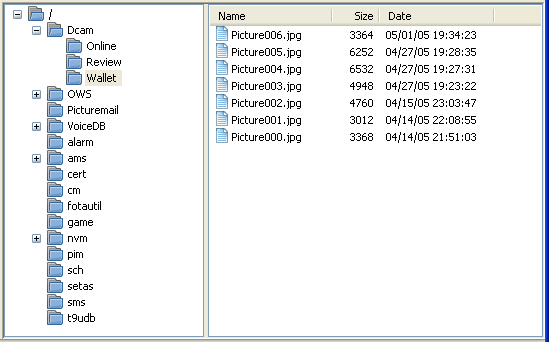
\includegraphics[width=130mm]{images/filesystem}}
  \caption{The concept of a file system: files and folders}
\end{figure}
The concept of a database table is really just like a spreadsheet,
with rows and columns.

\begin{figure}[h!]
  \centering
  \fbox{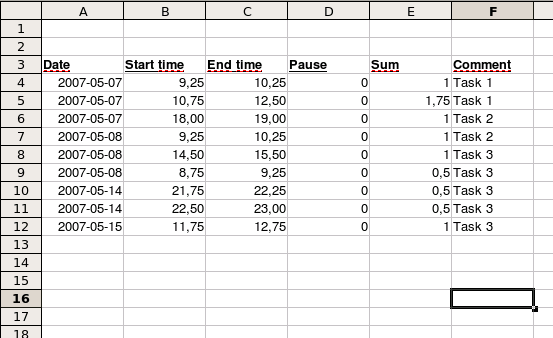
\includegraphics[width=130mm]{images/spreadsheet.png}}
  \caption{Information stored in rows and columns is a natural to keep information sorted.}
\end{figure}
  
Don't look at these images too closely, just keep the concepts in
mind.  So how do these two concepts form the basis of the Content
Management concept?  Basically when you are talking about content
management there two parts.  The first part is the actual file, or
piece of content.  The second part is the information about that piece
of content.  So what is common information people keep about a piece
of content.  Well some obvious information to store about a document
might be:

\begin{itemize}  
\item The author of the document
\item The size of the document
\item The type of document: word, pdf, spreadsheet, power-point
\end{itemize}

However, we might want to store even more information about a piece of
content.  We might want to say WHO can access the document.  This is
often a very important piece of information about the document.  Think
about your employement contract... you wouldn't want all your
colleagues to know how much you make would you?
  
So up to now we are really talking about two kinds of information.
The information inside the document and the information \emph{ABOUT}
the document.  People often use the word \emph{Content} to refer to
the information that is \emph{inside} the document and \emph{Metadata}
to refer to the information \emph{about} the document.  Lets look at
an picture to help us conceptualize this.

\begin{figure}[h!]
  \centering
  \fbox{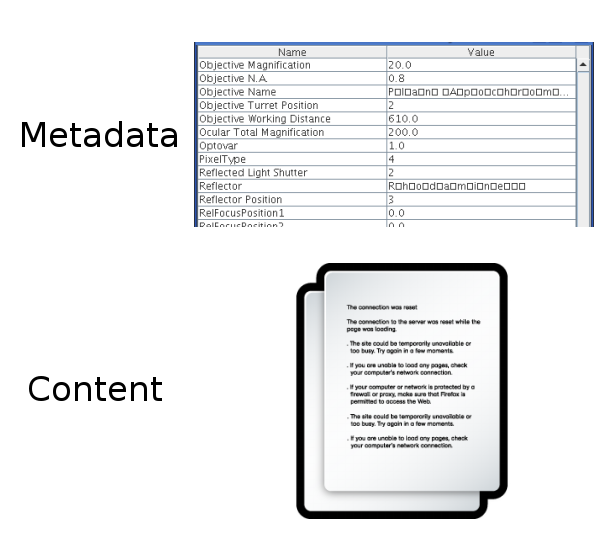
\includegraphics[width=130mm]{images/contentAndMetadata.png}}
  \caption{The concept of a file system: files and folders}
\end{figure}
  
So that is the essence of Content Management.  You have content, a
document, file, etc... and you have information about that document,
metadata.

\clearpage